\documentclass{article}
\usepackage{tikz}
\usepackage[utf8]{inputenc}
\usetikzlibrary{arrows,automata}
\usepackage[all]{xy}

\title{Práctica 3: Autómatas finitos}
\author{}
\date{November 2014}

\begin{document}

\maketitle

\section*{Ejercicio 1:}
Obtener un AFD capaz de aceptar las cadenas $u\in\{0,1\}^*$, que contengan simultáneamente las subcadenas 000 y 111.
\begin{center}
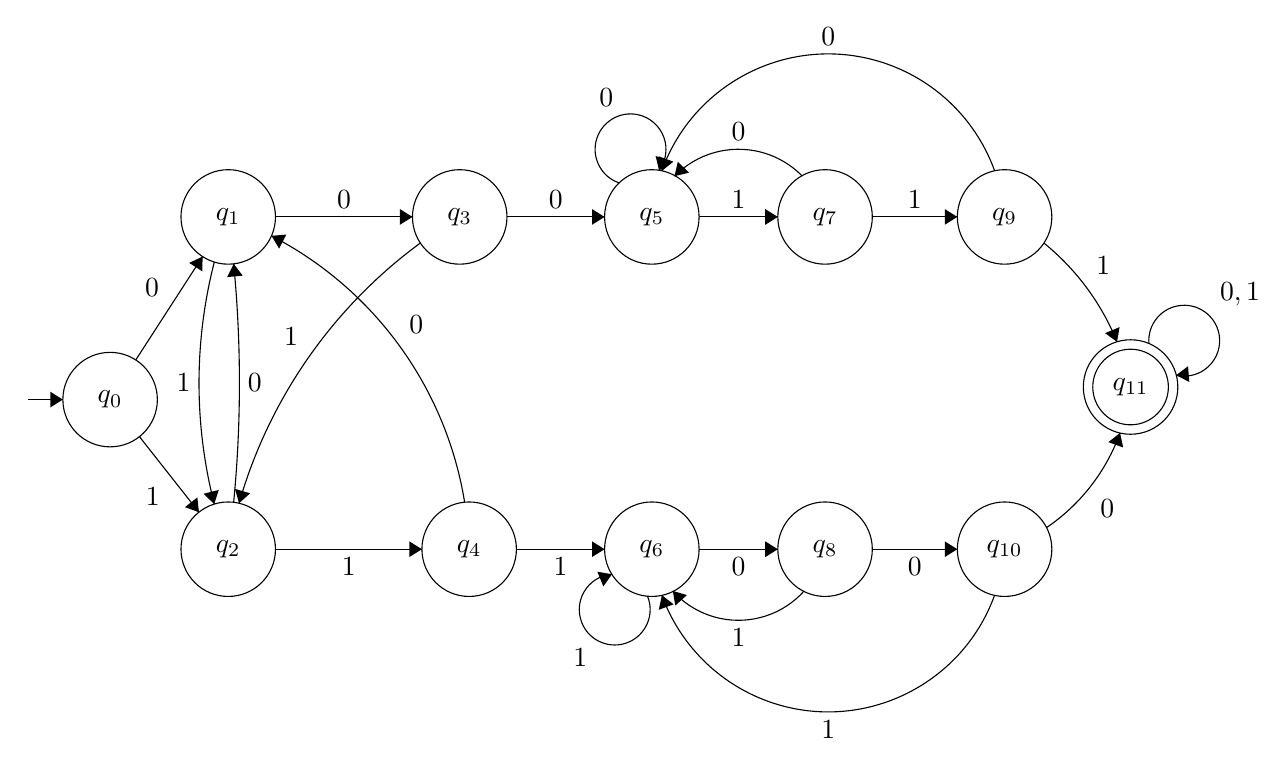
\begin{tikzpicture}[scale=0.2]
\tikzstyle{every node}+=[inner sep=0pt]
\draw [black] (5.9,-30.6) circle (3);
\draw (5.9,-30.6) node {$q_0$};
\draw [black] (13.4,-19) circle (3);
\draw (13.4,-19) node {$q_1$};
\draw [black] (13.4,-40.1) circle (3);
\draw (13.4,-40.1) node {$q_2$};
\draw [black] (28.1,-19) circle (3);
\draw (28.1,-19) node {$q_3$};
\draw [black] (28.7,-40.1) circle (3);
\draw (28.7,-40.1) node {$q_4$};
\draw [black] (40.3,-19) circle (3);
\draw (40.3,-19) node {$q_5$};
\draw [black] (40.3,-40.1) circle (3);
\draw (40.3,-40.1) node {$q_6$};
\draw [black] (51.3,-19) circle (3);
\draw (51.3,-19) node {$q_7$};
\draw [black] (62.7,-19) circle (3);
\draw (62.7,-19) node {$q_9$};
\draw [black] (70.7,-29.8) circle (3);
\draw (70.7,-29.8) node {$q_{11}$};
\draw [black] (70.7,-29.8) circle (2.4);
\draw [black] (62.7,-40.1) circle (3);
\draw (62.7,-40.1) node {$q_{10}$};
\draw [black] (51.3,-40.1) circle (3);
\draw (51.3,-40.1) node {$q_8$};
\draw [black] (7.53,-28.08) -- (11.77,-21.52);
\fill [black] (11.77,-21.52) -- (10.92,-21.92) -- (11.76,-22.46);
\draw (9.03,-23.48) node [left] {$0$};
\draw [black] (7.76,-32.95) -- (11.54,-37.75);
\fill [black] (11.54,-37.75) -- (11.44,-36.81) -- (10.65,-37.43);
\draw (9.09,-36.77) node [left] {$1$};
\draw [black] (16.4,-19) -- (25.1,-19);
\fill [black] (25.1,-19) -- (24.3,-18.5) -- (24.3,-19.5);
\draw (20.75,-18.5) node [above] {$0$};
\draw [black] (31.1,-19) -- (37.3,-19);
\fill [black] (37.3,-19) -- (36.5,-18.5) -- (36.5,-19.5);
\draw (34.2,-18.5) node [above] {$0$};
\draw [black] (16.4,-40.1) -- (25.7,-40.1);
\fill [black] (25.7,-40.1) -- (24.9,-39.6) -- (24.9,-40.6);
\draw (21.05,-40.6) node [below] {$1$};
\draw [black] (31.7,-40.1) -- (37.3,-40.1);
\fill [black] (37.3,-40.1) -- (36.5,-39.6) -- (36.5,-40.6);
\draw (34.5,-40.6) node [below] {$1$};
\draw [black] (0.7,-30.6) -- (2.9,-30.6);
\fill [black] (2.9,-30.6) -- (2.1,-30.1) -- (2.1,-31.1);
\draw [black] (13.746,-21.98) arc (5.52961:-5.52961:78.562);
\fill [black] (13.75,-21.98) -- (13.33,-22.82) -- (14.32,-22.73);
\draw (14.61,-29.55) node [right] {$0$};
\draw [black] (12.515,-37.235) arc (-165.60992:-194.39008:30.922);
\fill [black] (12.51,-37.23) -- (12.8,-36.34) -- (11.83,-36.58);
\draw (11.04,-29.55) node [left] {$1$};
\draw [black] (16.147,-20.202) arc (62.66991:9.22321:23.231);
\fill [black] (16.15,-20.2) -- (16.63,-21.01) -- (17.09,-20.12);
\draw (24.87,-25.82) node [right] {$0$};
\draw [black] (14.087,-37.181) arc (163.9934:126.2781:31.155);
\fill [black] (14.09,-37.18) -- (14.79,-36.55) -- (13.83,-36.27);
\draw (17.87,-26.6) node [left] {$1$};
\draw [black] (43.3,-19) -- (48.3,-19);
\fill [black] (48.3,-19) -- (47.5,-18.5) -- (47.5,-19.5);
\draw (45.8,-18.5) node [above] {$1$};
\draw [black] (54.3,-19) -- (59.7,-19);
\fill [black] (59.7,-19) -- (58.9,-18.5) -- (58.9,-19.5);
\draw (57,-18.5) node [above] {$1$};
\draw [black] (43.3,-40.1) -- (48.3,-40.1);
\fill [black] (48.3,-40.1) -- (47.5,-39.6) -- (47.5,-40.6);
\draw (45.8,-40.6) node [below] {$0$};
\draw [black] (54.3,-40.1) -- (59.7,-40.1);
\fill [black] (59.7,-40.1) -- (58.9,-39.6) -- (58.9,-40.6);
\draw (57,-40.6) node [below] {$0$};
\draw [black] (70.032,-32.717) arc (-19.87043:-55.80248:12.343);
\fill [black] (70.03,-32.72) -- (69.29,-33.3) -- (70.23,-33.64);
\draw (68.74,-37.5) node [right] {$0$};
\draw [black] (65.195,-20.657) arc (50.93147:22.12624:15.692);
\fill [black] (69.84,-26.93) -- (70,-26) -- (69.08,-26.38);
\draw (68.5,-22.11) node [right] {$1$};
\draw [black] (40.93,-16.076) arc (160.18546:19.81454:11.235);
\fill [black] (40.93,-16.08) -- (41.67,-15.49) -- (40.73,-15.15);
\draw (51.5,-8.15) node [above] {$0$};
\draw [black] (41.745,-16.411) arc (135.6824:44.3176:5.668);
\fill [black] (41.74,-16.41) -- (42.66,-16.19) -- (41.95,-15.49);
\draw (45.8,-14.2) node [above] {$0$};
\draw [black] (38.233,-16.842) arc (251.49548:-36.50452:2.25);
\draw (37.41,-12.02) node [above] {$0$};
\fill [black] (40.76,-16.05) -- (41.48,-15.45) -- (40.54,-15.13);
\draw [black] (40.022,-43.075) arc (22.3925:-265.6075:2.25);
\draw (35.76,-46.35) node [below] {$1$};
\fill [black] (37.77,-41.69) -- (36.84,-41.53) -- (37.22,-42.46);
\draw [black] (49.974,-42.751) arc (-41.89561:-138.10439:5.608);
\fill [black] (41.63,-42.75) -- (41.79,-43.68) -- (42.53,-43.01);
\draw (45.8,-45.11) node [below] {$1$};
\draw [black] (71.864,-27.048) arc (184.81508:-103.18492:2.25);
\draw (76.35,-23.94) node [right] {$0,1$};
\fill [black] (73.59,-29.05) -- (74.43,-29.48) -- (74.35,-28.48);
\draw [black] (62.064,-43.023) arc (-19.92932:-160.07068:11.237);
\fill [black] (40.94,-43.02) -- (40.74,-43.95) -- (41.68,-43.6);
\draw (51.5,-50.93) node [below] {$1$};
\end{tikzpicture}
\end{center}
En primer lugar vamos del estado $q_0$ a $q_1, q_2$ con un 0 o con un 1, ahora si se introduce un valor que rompa la cadena 000 o 111 se vuelve al inicio de la cadena para posteriormente seguir con los estados $q_5, q_6$ que continuan con la cadena opuesta a la leida con la obligación de tener que leerse completa puesto que si es un valor distinto volvemos al principio de la siguiente subcadena.
\section*{Ejercicio 2:}
Obtener un AFD equivalente al siguiente AFND:
\begin{center}
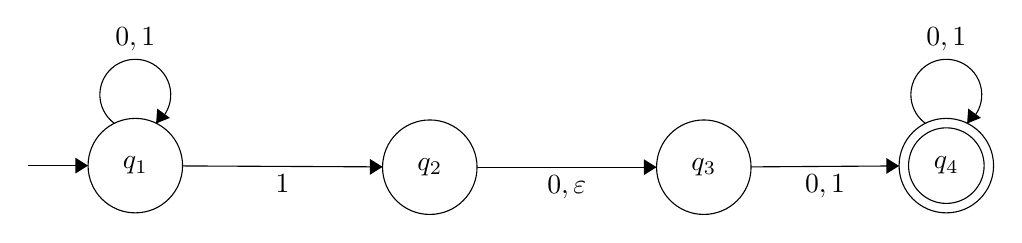
\begin{tikzpicture}[scale=0.2]
\tikzstyle{every node}+=[inner sep=0pt]
\draw [black] (18.2,-27.1) circle (3);
\draw (18.2,-27.1) node {$q_1$};
\draw [black] (36.9,-27.2) circle (3);
\draw (36.9,-27.2) node {$q_2$};
\draw [black] (54.3,-27.2) circle (3);
\draw (54.3,-27.2) node {$q_3$};
\draw [black] (69.7,-27.1) circle (3);
\draw (69.7,-27.1) node {$q_4$};
\draw [black] (69.7,-27.1) circle (2.4);
\draw [black] (11.4,-27.1) -- (15.2,-27.1);
\fill [black] (15.2,-27.1) -- (14.4,-26.6) -- (14.4,-27.6);
\draw [black] (16.877,-24.42) arc (234:-54:2.25);
\draw (18.2,-19.85) node [above] {$0,1$};
\fill [black] (19.52,-24.42) -- (20.4,-24.07) -- (19.59,-23.48);
\draw [black] (21.2,-27.12) -- (33.9,-27.18);
\fill [black] (33.9,-27.18) -- (33.1,-26.68) -- (33.1,-27.68);
\draw (27.55,-27.66) node [below] {$1$};
\draw [black] (39.9,-27.2) -- (51.3,-27.2);
\fill [black] (51.3,-27.2) -- (50.5,-26.7) -- (50.5,-27.7);
\draw (45.6,-27.7) node [below] {$0,\varepsilon$};
\draw [black] (57.3,-27.18) -- (66.7,-27.12);
\fill [black] (66.7,-27.12) -- (65.9,-26.62) -- (65.9,-27.62);
\draw (62,-27.66) node [below] {$0,1$};
\draw [black] (68.377,-24.42) arc (234:-54:2.25);
\draw (69.7,-19.85) node [above] {$0,1$};
\fill [black] (71.02,-24.42) -- (71.9,-24.07) -- (71.09,-23.48);
\end{tikzpicture}
\end{center}
Solución:\\
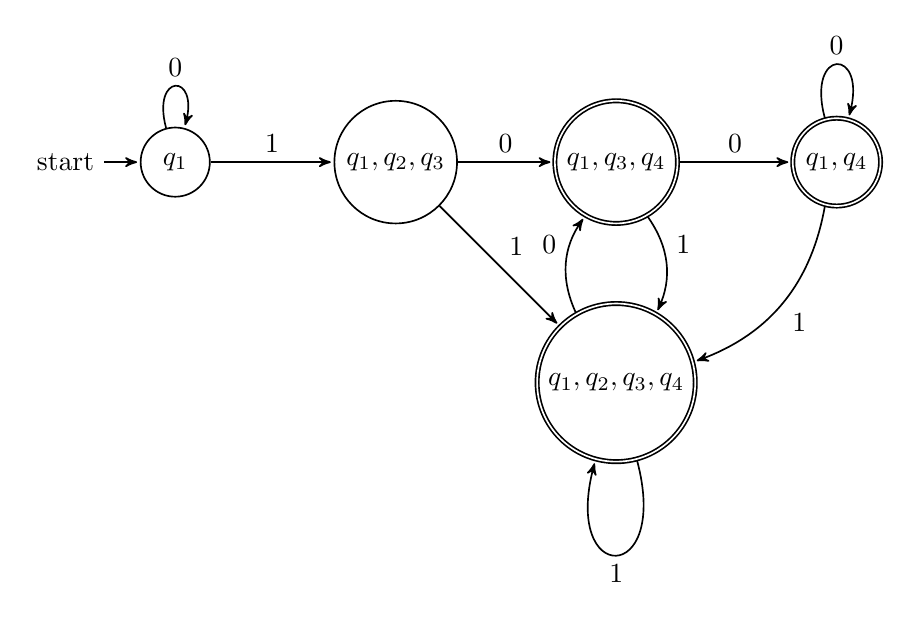
\begin{tikzpicture}[->,>=stealth',shorten >=1pt,auto,node distance=2.8cm,semithick]

  \node[initial,state] (A)                    {$q_1$};
  \node[state]         (B) [right of=A] {$q_1,q_2,q_3$};
  \node[state,accepting]         (C) [right of=B] {$q_1,q_3, q_4$};
  \node[state,accepting]         (D) [right of=C] {$q_1,q_4$};
  \node[state,accepting]         (E) [below of=C]       {$q_1,q_2,q_3,q_4$};

  \path (A) edge		[loop above]		node {0} (A)
  		(A) edge              node {1} (B)
        (B) edge node {0} (C)
            edge              node {1} (E)
        (C) edge              node {0} (D)
            edge [bend left]  node {1} (E)
        (D) edge [bend left] node {1} (E)
            edge [loop above] node {0} (A)
        (E) edge [loop below]  node {1} (E)
        		edge [bend left] node {0} (C);
\end{tikzpicture}
 \begin{itemize}
 \item Comenzamos por $q_1$ con un 0 se dirige a si mismo y con un 1 genera el estado $q_1,q_2,q_3$ puesto que $q_2$ admite una palabra vacia que lleva a $q_3$.
 \item $q_1,q_2,q_3$ con un 0 genera el estado, final puesto que contiene a $q_4$, $q_1,q_3,q_4$ debido a que $q_3$ va a $q_4$ con un 0 o un 1, y con un 1 genera un estado con $q_1,q_2,q_3,q_4$ también final.
 \item $q_1,q_3,q_4$ con un 0 genera el estado $q_1,q_4$ ya que el estado $q_3$ se pierde, y con un 1 vuelve a $q_1,q_2,q_3,q_4$.
 \item $q_1,q_2,q_3,q_4$ con un 1 vuelve a él mismo y con un 0 regresa a $q_1,q_3,q_4$.
 \item Por último el estado final $q_1,q_4$ con un 0 va a él mismo y con un 1 vuelve al estado $q_1,q_2,q_3,q_4$.
 \end{itemize}
\section*{Ejercicio 3:}
Construir un AFND a partir de cada una de las siguientes expresiones regulares:
$$(aa)^*b^*$$
\begin{center}
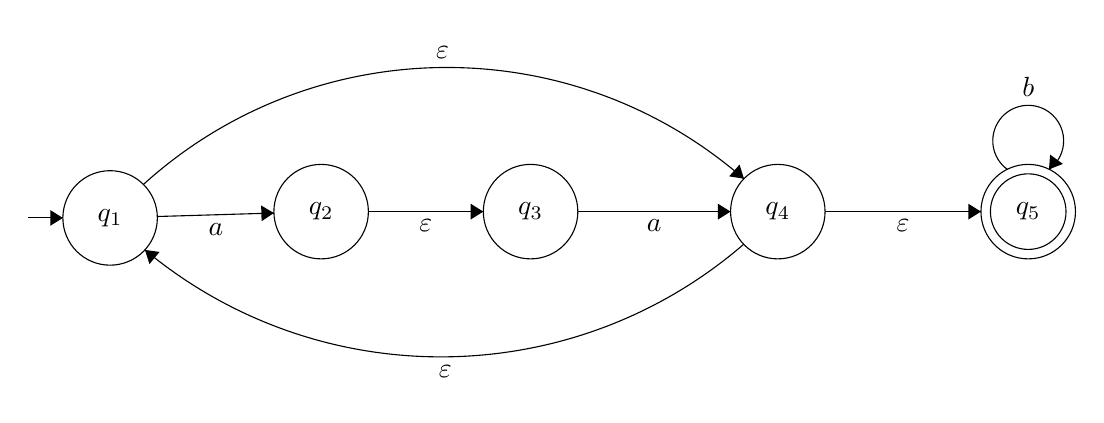
\begin{tikzpicture}[scale=0.2]
\tikzstyle{every node}+=[inner sep=0pt]
\draw [black] (5.9,-30.6) circle (3);
\draw (5.9,-30.6) node {$q_1$};
\draw [black] (19.3,-30.2) circle (3);
\draw (19.3,-30.2) node {$q_2$};
\draw [black] (32.6,-30.2) circle (3);
\draw (32.6,-30.2) node {$q_3$};
\draw [black] (48.3,-30.2) circle (3);
\draw (48.3,-30.2) node {$q_4$};
\draw [black] (64.2,-30.2) circle (3);
\draw (64.2,-30.2) node {$q_5$};
\draw [black] (64.2,-30.2) circle (2.4);
\draw [black] (0.7,-30.6) -- (2.9,-30.6);
\fill [black] (2.9,-30.6) -- (2.1,-30.1) -- (2.1,-31.1);
\draw [black] (8.014,-28.474) arc (132.16897:48.91205:28.702);
\fill [black] (46.15,-28.11) -- (45.87,-27.21) -- (45.21,-27.96);
\draw (27.01,-20.54) node [above] {$\varepsilon$};
\draw [black] (46.133,-32.273) arc (-49.19247:-129.72651:29.418);
\fill [black] (8.11,-32.63) -- (8.4,-33.53) -- (9.04,-32.76);
\draw (27.19,-39.93) node [below] {$\varepsilon$};
\draw [black] (8.9,-30.51) -- (16.3,-30.29);
\fill [black] (16.3,-30.29) -- (15.49,-29.81) -- (15.52,-30.81);
\draw (12.62,-30.93) node [below] {$a$};
\draw [black] (22.3,-30.2) -- (29.6,-30.2);
\fill [black] (29.6,-30.2) -- (28.8,-29.7) -- (28.8,-30.7);
\draw (25.95,-30.7) node [below] {$\varepsilon$};
\draw [black] (35.6,-30.2) -- (45.3,-30.2);
\fill [black] (45.3,-30.2) -- (44.5,-29.7) -- (44.5,-30.7);
\draw (40.45,-30.7) node [below] {$a$};
\draw [black] (51.3,-30.2) -- (61.2,-30.2);
\fill [black] (61.2,-30.2) -- (60.4,-29.7) -- (60.4,-30.7);
\draw (56.25,-30.7) node [below] {$\varepsilon$};
\draw [black] (62.877,-27.52) arc (234:-54:2.25);
\draw (64.2,-22.95) node [above] {$b$};
\fill [black] (65.52,-27.52) -- (66.4,-27.17) -- (65.59,-26.58);
\end{tikzpicture}
\end{center}
$$a(b+a)^*b$$
\begin{center}
\begin{tikzpicture}[scale=0.2]
\tikzstyle{every node}+=[inner sep=0pt]
\draw [black] (9.2,-25.8) circle (3);
\draw (9.2,-25.8) node {$q_1$};
\draw [black] (22,-25.8) circle (3);
\draw (22,-25.8) node {$q_2$};
\draw [black] (33.5,-25.8) circle (3);
\draw (33.5,-25.8) node {$q_3$};
\draw [black] (42.4,-16.1) circle (3);
\draw (42.4,-16.1) node {$q_4$};
\draw [black] (54.7,-16.1) circle (3);
\draw (54.7,-16.1) node {$q_5$};
\draw [black] (42.4,-35.2) circle (3);
\draw (42.4,-35.2) node {$q_6$};
\draw [black] (54.7,-35.2) circle (3);
\draw (54.7,-35.2) node {$q_7$};
\draw [black] (61.9,-25.8) circle (3);
\draw (61.9,-25.8) node {$q_8$};
\draw [black] (73.7,-25.8) circle (3);
\draw (73.7,-25.8) node {$q_9$};
\draw [black] (73.7,-25.8) circle (2.4);
\draw [black] (1.8,-25.8) -- (6.2,-25.8);
\fill [black] (6.2,-25.8) -- (5.4,-25.3) -- (5.4,-26.3);
\draw [black] (12.2,-25.8) -- (19,-25.8);
\fill [black] (19,-25.8) -- (18.2,-25.3) -- (18.2,-26.3);
\draw (15.6,-26.3) node [below] {$a$};
\draw [black] (25,-25.8) -- (30.5,-25.8);
\fill [black] (30.5,-25.8) -- (29.7,-25.3) -- (29.7,-26.3);
\draw (27.75,-26.3) node [below] {$\varepsilon$};
\draw [black] (35.53,-23.59) -- (40.37,-18.31);
\fill [black] (40.37,-18.31) -- (39.46,-18.56) -- (40.2,-19.24);
\draw (38.49,-22.41) node [right] {$\varepsilon$};
\draw [black] (35.56,-27.98) -- (40.34,-33.02);
\fill [black] (40.34,-33.02) -- (40.15,-32.1) -- (39.42,-32.78);
\draw (37.42,-31.97) node [left] {$\varepsilon$};
\draw [black] (32.532,-22.969) arc (-168.49027:-322.33707:11.662);
\fill [black] (32.53,-22.97) -- (32.86,-22.09) -- (31.88,-22.29);
\draw (38.18,-9.53) node [above] {$\varepsilon$};
\draw [black] (53.399,-37.894) arc (-33.16525:-194.65939:11.649);
\fill [black] (32.38,-28.57) -- (31.69,-29.22) -- (32.66,-29.47);
\draw (38,-42.68) node [below] {$\varepsilon$};
\draw [black] (45.4,-35.2) -- (51.7,-35.2);
\fill [black] (51.7,-35.2) -- (50.9,-34.7) -- (50.9,-35.7);
\draw (48.55,-35.7) node [below] {$b$};
\draw [black] (45.4,-16.1) -- (51.7,-16.1);
\fill [black] (51.7,-16.1) -- (50.9,-15.6) -- (50.9,-16.6);
\draw (48.55,-16.6) node [below] {$a$};
\draw [black] (56.49,-18.51) -- (60.11,-23.39);
\fill [black] (60.11,-23.39) -- (60.04,-22.45) -- (59.23,-23.05);
\draw (57.72,-22.34) node [left] {$\varepsilon$};
\draw [black] (56.52,-32.82) -- (60.08,-28.18);
\fill [black] (60.08,-28.18) -- (59.19,-28.51) -- (59.99,-29.12);
\draw (58.87,-31.91) node [right] {$\varepsilon$};
\draw [black] (64.9,-25.8) -- (70.7,-25.8);
\fill [black] (70.7,-25.8) -- (69.9,-25.3) -- (69.9,-26.3);
\draw (67.8,-26.3) node [below] {$b$};
\draw [black] (61.988,-28.796) arc (-2.59646:-177.40354:20.059);
\fill [black] (61.99,-28.8) -- (61.45,-29.57) -- (62.45,-29.62);
\draw (41.95,-48.45) node [below] {$\varepsilon$};
\end{tikzpicture}
\end{center}
\pagebreak
b) Transformar los AFND’s obtenidos en el apartado anterior a AFD’s.
$$(aa)*b^*$$
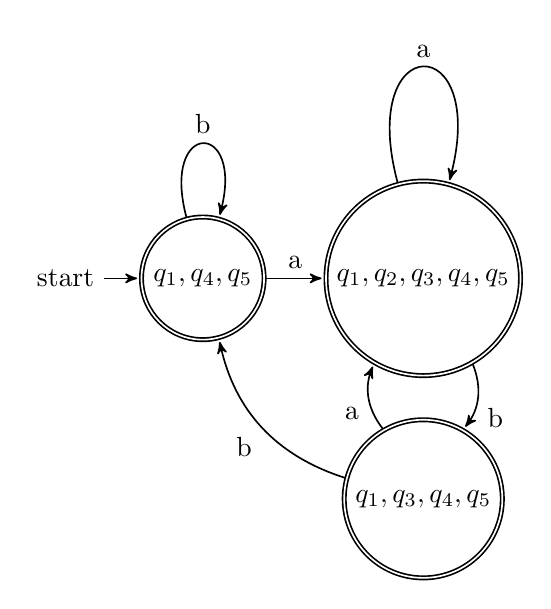
\begin{tikzpicture}[->,>=stealth',shorten >=1pt,auto,node distance=2.8cm,semithick]

  \node[initial,state,accepting] (A)                    {$q_1,q_4,q_5$};
  \node[state,accepting]         (B) [right of=A] {$q_1,q_2,q_3,q_4,q_5$};
  \node[state,accepting]         (C) [below of=B] {$q_1,q_3, q_4,q_5$};

  \path (A) edge		[loop above]		node {b} (A)
  		(A) edge              node {a} (B)
        (B) edge [bend left] node {b} (C)
            edge  [loop above]            node {a} (E)
        (C) edge   [bend left]           node {a} (B)
            edge [bend left]  node {b} (A);
\end{tikzpicture}
$$a(b+a)^*b$$
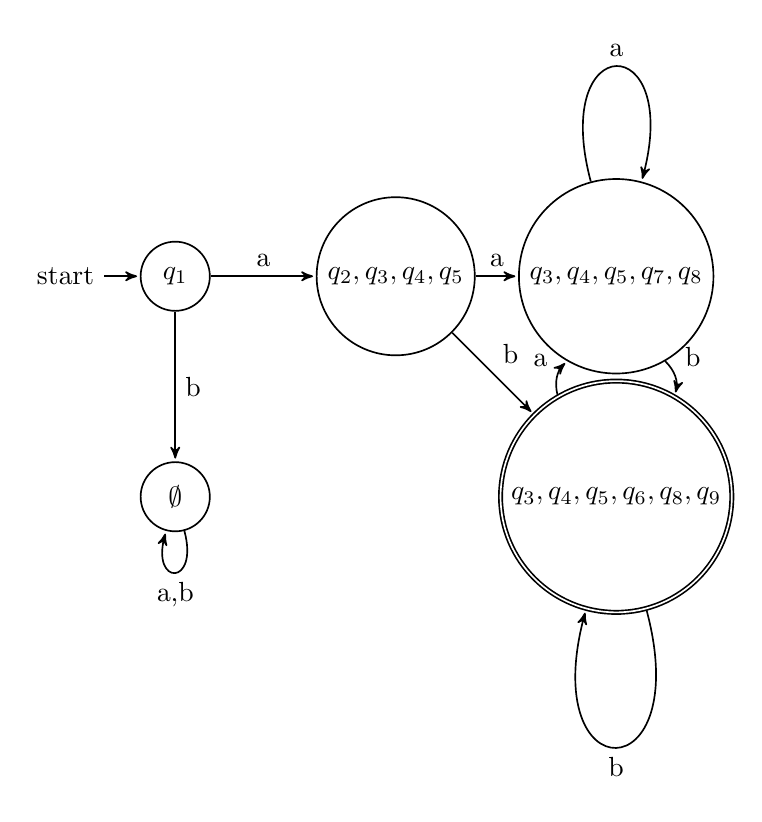
\begin{tikzpicture}[->,>=stealth',shorten >=1pt,auto,node distance=2.8cm,semithick]

  \node[initial,state] (A)                    {$q_1$};
  \node[state]         (B) [right of=A] {$q_2,q_3,q_4,q_5$};
  \node[state]         (C) [right of=B] {$q_3,q_4, q_5,q_7,q_8$};
  \node[state,accepting]         (D) [below of=C] {$q_3,q_4,q_5,q_6,q_8,q_9$};
  \node[state]         (E) [below of=A]       {$\emptyset$};

  \path (A) edge		node {a} (B)
  		(A) edge              node {b} (E)
        (B) edge node {a} (C)
            edge    node {b} (D)
        (C) edge [bend left]             node {b} (D)
            edge [loop above]  node {a} (C)
        (D) edge [bend left] node {a} (C)
            edge [loop below] node {b} (D)
        (E) edge [loop below]  node {a,b} (E);
\end{tikzpicture}
\end{document}
